\subsection{Program-event rate and round duration across windows}\label{app:latest-event-rates}

\Cref{fig:fw-latest-event-rates} consolidates four retained windows with
raw event counts and wall durations and a fresh matched 20-round capture.
Each rate divides that window's total events by its total completed-round
wall time; each mean duration divides the same time by 20. Sources lacking
raw duration, or lacking 20 consecutive rounds, are excluded rather than
imputed. The last of those five windows, rounds 3001--3020, records 12 program events
over \num{1809.50}\,s and no adapter admissions. Its summary event counts
match the promotion journal. Scope and window-separation rules follow
\cref{sec:method-status}.

\begin{figure*}[!t]
  \setlength{\abovecaptionskip}{4pt}
  \centering
  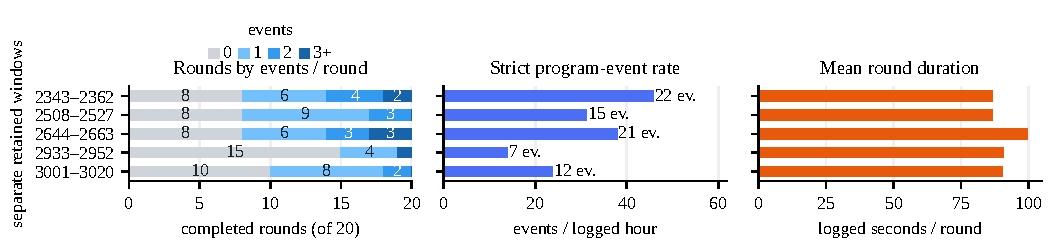
\includegraphics[width=\linewidth,height=1.65in,keepaspectratio]{figures/fig_fw_latest_event_rates.pdf}
  \caption{\textbf{Event distributions, program-event rates and round durations across retained 20-round windows.}
  Each row is a separate capture of 20 consecutive completed rounds with logged wall times.
  Left: completed rounds grouped by 0, 1, 2 or 3+ strict training-program incumbent events.
  Center: strict training-program incumbent events divided by total logged round time (events per hour), with total
  window event counts annotated. Right: mean completed-round duration (seconds) over the 20 rounds, including
  all within-round work and waits. Windows are displayed separately; program events are distinct
  from adapter admissions. Scope: \cref{sec:method-status}.}
  \label{fig:fw-event-distribution}
  \label{fig:fw-latest-event-rates}
\end{figure*}
